\documentclass[12pt,fleqn]{article}\usepackage{../common}
\begin{document}
Ders 2

Sureklilik

Tanim

$S \subset \mathbb{R}$, $f: S \to \mathbb{R}$ bir fonksiyon olsun, ve $c
\in S$ bir sayi olsun. 
``$f$'in $c$'de surekli oldugu'' soylenir, su durumda: Eger her
$\epsilon>0$ icin bir $\delta > 0$ var ise, oyle ki ne zaman $x \in S$ ve $|x-c| < \delta$
ise, o zaman $|f(x) - f(c)| < \epsilon$ dogrudur. 

Eger  $f: S \to \mathbb{R}$ her $c \in S$ icin dogru ise, yani bir $c$
noktasi degil tum $c$'ler icin gecerli ise, o zaman $f$'in surekli oldugunu
soyleriz. Yani nokta belirtmeye ihtiyac kalmaz. 

Ustteki tanim Analizde dogru anlasilmasi gereken en onemli teorilerden
biridir, ve tam anlamasi pek kolay olmayabilir. Dikkat edilirse $\delta$,
hem $\epsilon$'a hem de $c$'ye bagli. Yani her $c \in S$ icin ayni $\delta$ secilmiyor.

Ayrica surekli fonksiyonlarin taniminin limitlerin tanimina benziyor olmasi 
raslanti degil, surekli fonksiyonlarin onemli bir ozelligi zaten onlarin
duzgun limitleri olmalari.

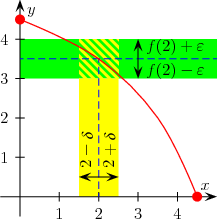
\includegraphics[height=4cm]{2_5.png}

Tanimin islemesinde mutlak deger (absolute value, $||$ isareti) kritik bir rol
oynuyor. Grafiksel olarak soyle gosterebiliriz. Bir fonksiyonun degerleri
etrafinda, yukari, asagi olmak uzere $\epsilon$ kadar bir pencere
tanimliyoruz (yesil olarak gorulen bolum). Simdi ornekte $c=2$ etrafinda,
yani $x$ bazinda oyle bir baska pencere tanimlayalim ki, bu penceredeki
degerler tamamen yesil kisima tekabul eden degerlerin icinde kalsin. Bu
sekilde tek bir pencere bulabildigimiz anda is tamamdir. Ve bunu tum
$\epsilon > 0$ icin yapabiliyorsak, o fonksiyon surekli demektir. 

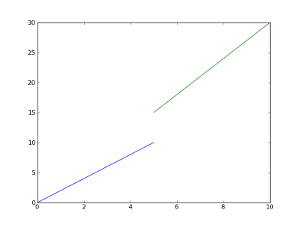
\includegraphics[height=4cm]{2_4.png}

Diger yandan ustteki grafikte gosterilen 

\[ 
f(x) = 
\left\{ \begin{array}{ll}
x < 5 & 2x \\
x \ge 5 & 3x
\end{array} \right.
 \]

fonksiyonu surekli degildir. Eger $c=5$ etrafinda $\epsilon = 4$ alirsak
mesela, bu pencereye tekabul eden bir $\delta$ bulamayiz. Fakat su
fonksiyon sureklidir.

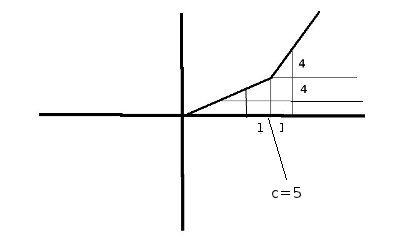
\includegraphics[height=4cm]{2_3.png}

\[ 
f(x) = 
\left\{ \begin{array}{ll}
x < 5 & 2x \\
x \ge 5 & 3x + 10
\end{array} \right.
 \]

Fonksiyonun puruzsuz (smooth) olmadigina dikkat, yani iki parcali bir
fonksiyon, kesikli bir sekilde tanimli, ama yine de surekli. 

Esit Sureklilik (Uniform Continuity) 

Sureklilik taniminda $\delta$'nin $c$ noktasina bagli oldugunu
soylemistik. Ama bazi durumlarda $\delta$'nin bagimsiz olmasi daha
faydalidir. 

Tanim

$S \subset \mathbb{R}$, $f:S \to \mathbb{R}$ bir fonksiyon olsun. Farz edelim ki her $\epsilon > 0$ icin 
bir $\delta > 0$ mevcut, ki $x,c \in S$ ve $|x-c| < \delta$ oldugu zaman, $|f(x) - f(c)| < \epsilon$. 
Bu durumlarda fonksiyona esit surekli denir. 

Esit Surekli bir fonksiyonun (normal) surekli bir fonksiyon olacagini
gormek zor olmaz. Buradaki tek fark her secilen $\epsilon > 0$ icin oyle
bir $\delta > 0$ seciyoruz ki bu $\delta$ her $c \in S$ icin ise
yariyor. Yani bu yeni tanima gore artik $\delta$, $c$'ye bagli degil,
sadece $\epsilon$'a bagli. Tanimin yapildigi arka plan, bolge (domain)
bir fark yaratacak. Daha buyuk bir kumede esit surekli olmayan bir
fonksiyon, daha ufak bir kume icinde esit surekli haline gelebilecek. 

Lipschitz Surekliligi 

Tanim 

$f:S \to \mathbb{R}$ bir fonksiyon olsun, oyle ki $S$ icindeki her $x,y$
icin bir $K$ sayisi mevcut, ve tum bunlarla alttaki esitsizlik 
dogru

\[ |f(x) - f(y)| \le K|x-y| \]

O zaman $f$'e Lipschitz Surekli adi verilir. 

Cok genis bir fonksiyon kategorisi Lipschitz sureklidir. Fakat dikkat edin,
aynen esit sureklilikte oldugu gibi Lipschitz surekliliginde de fonksiyonun
tanimlandigi bolge (domain) cok onemlidir. Simdi ``surekli'' kelimesini
kullanmamizin dogrulugunu kontrol edelim. 

Teori 

Her Lipschitz surekli fonksiyon, ayni zamanda esit surekli bir
fonksiyondur. 

Ispat

$f: S \to \mathbb{R}$ oldugunu kabul edelim, ve oyle bir $K$ sayisi olsun ki $S$
icindeki her $x$ ve $y$ icin $f(x) - f(y)| \le K|x-y|$. Bu Lipschitz sureklilik
taniminin bir tekrari. Bir $\epsilon > 0$ secelim. Sonra $\delta =
\epsilon / K$ alalim. 
$|x-y| < \delta$ olacak sekilde her $x,y \in S$ icin 

\[ |f(x) - f(y)| \le K|x-y| < K\delta = K \frac{ \epsilon}{K} = \epsilon \]

Birinci esitsizlik Lipschitz tanimindan geliyor. Bu esitsizligin sag
tarafinda diger bildiklerimizi yerine koyunca, $\epsilon$ elde ediyoruz. 

Tamamlilik (Completeness) 

Tanim

Bir metrik uzayi $(X,d)$ tamamdir (complete) eger $X$ alanindaki her Cauchy
serisi (o da $X$ icinde olan) bir ogeye yaklasiyor ise. 

Ustteki tanimi onceki dersteki Cauchy tanimi ile birlestirirsek,
$\mathbb{R}$ uzayinin ``tamam'' oldugunu gorebiliriz. Cunku her Cauchy
dizisinin $\mathbb{R}$'de yakinlastigini biliyoruz, ayrica bir bir reel sayiya
yaklasildigini biliyoruz. Bu reel sayi $L$'in kendisi de zaten $\mathbb{R}$ icinde
olduguna gore, $\mathbb{R}$ uzayi tamamdir. 

Inf ve Sup

Sup

Eger $S$ kumesi ``yukaridan sinirlanmis (bounded from above)'' ise o zaman
$x \in S$ icin oyle bir $y$ var demektir ki her $x$ icin $x \le y$
olsun. Yani $S$ icindeki her deger bu $y$ degerinden kucuk olsun. Bu $x$
degerine $S$'in supremum'u da deniyor, ve $\sup\limits_{x \in S}(x)$ ya da
$sup\{x:x \in S\}$ olarak gosterilebiliyor. 

Inf

Benzer sekilde kumenin en alt siniri, yani infimum degeri $\inf\limits_{x
  \in S}(x)$ ya 
da $inf\{x:x \in
S\}$ olarak gosteriliyor. 

Eger elimizde bir seri (sequence) var ise o zaman sartlari biraz daha
gevsetmek iyidir, burada limit superior kavrami devreye girer. Inf ve sup
degerleri alti / ustu deger olamaz, ama limit superior oyle bir sayidir ki
onun sonrasinda sonlu (finite) / belli sayida kume ogesi olmasina izin
verilir. Limit superior aslinda bir serinin yaklastigi (converge) degerden
baskasi degildir. 

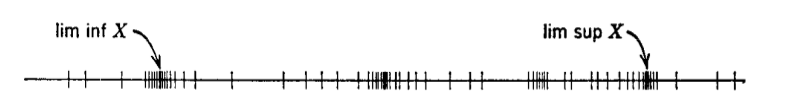
\includegraphics[height=1.5cm]{2_1.png}

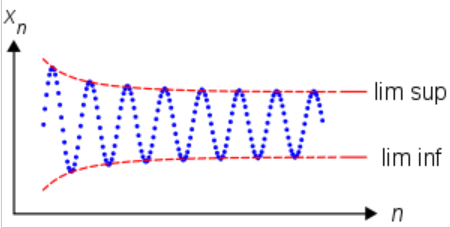
\includegraphics[height=3cm]{2_2.png}

Formel olarak diyelim ki $\{x_n\}$ bir seri, ve diyelim ki bir reel
sayi $S$ var, ki bu reel sayi su sartlari tatmin ediyor 
1) Her $\epsilon > 0$ icin bir $N$ var, oyle ki her $n>N$ icin $x_n
< S + \epsilon$ 
ve 2) her $\epsilon > 0$ ve $M>0$ icin bir  $n>M$ var ki $x_n
> S - \epsilon$. O 
zaman $S$ sayisina  $\{x_n\}$ serisinin limit superior'u denir. 

Bu tanimin soylemeye calistigi serinin yaklastigi degerden sonra ve once
sonlu buyuklukte (bir pencere tanimlarsak bu pencere icinde sonlu sayida
eleman olacaktir (sonsuz degil). Bu pencerenin tanimlanabiliyor olmasi,
onun makul bir noktada olmasini gerektirir, ki bu nokta da yaklasilan
degerden baskasi degildir. 

Limit inferior bunun tersidir, 

\[ \lim \inf x_n  = -\lim \sup(-x_n)\]

Vektor Uzaylari 

Her vektor uzayiyla ilintili olan bir tek buyukluk (scalar) kumesi vardir,
ve bu buyuklukler ile o uzayda carpim islemi tanimlanir. Soyut baglamda
calisilanlar icin bu buyukluklerin cebirsel bir alan (algebraic field -bir
soyut matematik kavrami-) uyesi olmasi yeterlidir. Fakat bu notlarda
kullanacagimiz buyuklukler ya reel sayilar, ya da kompleks sayilar
olacak. Bu iki olasilik arasinda hangisini kullandigimizi belli etmek icin
vektor uzayina ``reel vektor uzayi'' ya da ``kompleks vektoru uzayi''
diyebiliriz. Odagimiz ise cogunlukla reel vektor uzaylari olacak, kompleks
olanlari nadir kullanacagiz. Yani eger uzayin sekli soylenmemisse, onun
reel oldugunu farz edin. 

Tanim 

Vektor uzayi $X$, ``vektor'' denen ogeleri iceren bir kume, arti iki
operasyondan olusur. Ilk operasyon toplama, digeri carpmadir. Toplama
islemi iki vektor $x,y \in X$'i bir diger vektor $x+y \in X$ ile
bagdastirir. Carpma islemi $x \in X$ ve herhangi bir sayi, skalar $\alpha$
ile vektor $\alpha x$'i bagdastirir. 

$\theta$ sifir vektorudur. 

\[ 0 \ x = \theta, \ 1 \ x = x \]

[diger onsartlar atlandi, sirabagimsizlik (commutative) kurali, vs, toplam 7
tane]

Ornek

Herhalde vektor uzaylarina verilecek en basit ornek reel sayilar
kumesidir. Bu durumda kume elemanlari olan ``vektorler'' tek
boyutludur. Vektoru uzayi (dogal olarak) bir reel vektor uzayidir, toplama,
carpma reel sayilarin uzerinden tanimlidir. Sifir vektoru $\theta$, sifir
sayisidir. Bu uzaya reel kordinat uzayi, ya da basit ifadeyle ``reel cizgi
(real line)'' adi da verilebilir, $R^1$, ya da $R$ olarak gosterilir. 




\end{document}
